\documentclass[conference]{IEEEtran}
%Consideration: Language, Logic, Plotting
\usepackage{xcolor}
\usepackage{graphicx}
\usepackage{amsmath}
\usepackage{acronym}
\newacro{efim}[EFIM]{Equivalent Fisher Information Matrix}
\newacro{fim}[FIM]{Fisher Information Matrix}
\usepackage{bm}
\usepackage{amsthm}
%\usepackage{showframe}
%\usepackage{cite}
\newtheorem{theorem}{Theorem}
\newtheorem{lemma}{Lemma}
\newtheorem{definition}{Definition}
\newtheorem{remark}{Remark}

\DeclareMathOperator\tr{tr}
\DeclareMathOperator\diag{diag}
%conditional compiling here
\newif\ifshowdetail
\showdetailtrue
%\showdetailfalse
\begin{document}
\title{On the Temporal Cooperation Efficiency in Wireless Networks}
\author{\IEEEauthorblockN{Feng Zhao}
\IEEEauthorblockA{Department of Electronic Engineering\\
Graduate School at Shenzhen,\\
Tsinghua University, P.R. China\\
Email: zhaof17@mails.tsinghua.edu.cn}}
\maketitle
%\ead{zhaof17@mails.tsinghua.edu.cn}
%\address[rvt]{Department of Electronic Engineering, Tsinghua University, Beijing 100084}
\begin{abstract}
Cooperative localization technology utilizing previous estimated position of agents can significantly improve the localization accuracy.
Starting from Fisher information matrix, this paper describes the temporal decaying characteristics of localization error. 
With the method of continued fraction analysis, the exponential decaying property of localization error propagation speed is determined.
The characteristics of error propagation are further interpreted geometrically and validated by numerical results. 
%which gives insight on the relationship between localization error and cooperative information.
\end{abstract}
\begin{IEEEkeywords}
Cooperative localization, Fisher informaton matrix, Position error bound, Matrix algebra, Continued fraction
\end{IEEEkeywords}
\maketitle



\section{Introduction}
% no \IEEEPARstart
The acquisition of real-time target position is an important part of application in wireless communication technology. 
It has wide applications in personal navigation, battlefield surveillance and internet of vehicles~\cite{Win2011Network}. 
For situations where positions of multiple agents are required, 
cooperative localization technology based on distance measure information between agents can significantly improve the localization accuracy. 
However, localization error is unavoidable in cooperative localization network 
and it is a vital topic in this field to investigate the property of localization error bound.

There are many kinds of metric to describe the localization error bound 
including geometric dilution of precision~\cite{6237577}, root mean square error, 
cumulative distribution probability and \ac{fim}. 
Compared with other metrics, Fisher information matrix is the theoretical limit of localizations~\cite{LimitBound2}. 
There have been many papers investigating the property of localization error bound based on \ac{fim}. 
It is been shown that the average localization performance of a network is largely determined by the number of agents and the signal metric employed~\cite{7887727}. 
Some geometric interpretations of \ac{fim} decomposition is given and the efficiency of cooperation is analyzed~\cite{7962761}. 
Though the same metric \ac{fim} is employed, different decomposition techniques and interpretations exist. 
The inverse of \ac{fim} holds only approximately~\cite{7887727} 
and the series expansion is difficult  to analyze~\cite{7962761}. In this paper, 
we propose a novel mathematical method to analyze the cooperation efficiency and give reasonable geometric interpretations. 
Our results give insight on the relationship between localization error and cooperative information. 

The paper is organized as follows. Section \ref{systemModel} gives the basic model for our analysis. 
Section \ref{efficiency} derives the spatial positioning error bound (SPEB) for our scenario. 
Section \ref{geometry} gives geometric interpretation of our results. 
Section \ref{numerical} shows the simulated results and its comparison with the theoretical bound.

Throughout this paper, the superscript $[\cdot]^{\mathrm{T}}$ represents the transpose of its argument. 
We use $\bm{\mathrm{I}}_2$ for the two dimensional identity matrix. The zero matrix is denoted by $\bm{0}$, 
whose dimension depends on used condition. $\tr\{\cdot\}$ 
denotes the trace of a square matrix.
\begin{figure}
  \centering
\def\svgwidth{7cm}
\input{geometric_interpretation_v2.eps_tex}
\caption{One agent locating itself with information from anchors and previous time steps}
\label{f1}
\end{figure}
\section{System Model}\label{systemModel}
Consider a cooperative wireless network with one agent and several anchors. The anchors locate the agent at time $t_1,t_2,\dots,t_n$ via distance measurement. Also the agent can determine its position change through speed measurement. The position of the agent at different times can be stacked into a vector $\bm{\theta}=[\bm{p}_1,\dots,\bm{p}_n]^{\mathbf{T}}$.

We use \ac{fim} to evaluate the accuracy of estimation of $\bm{\theta}$~\cite{LimitBound2}. The \ac{fim} takes the following form
\begin{equation}
\bm{\mathrm{J}}(\bm{\theta})=\bm{\mathrm{J}}^\mathrm{A}(\bm{\theta})+\bm{\mathrm{J}}^\mathrm{C}(\bm{\theta})
\end{equation}
where $\bm{\mathrm{J}}^\mathrm{C}(\bm{\theta})$ in \eqref{eq:JC} represents the contribution of cooperation among adjacent times, $\bm{\mathrm{J}}^\mathrm{A}(\bm{\theta})$ represents the information from anchors. 
\begin{figure*}[t]
\begin{equation}\label{eq:JC}
\bm{\mathrm{J}}^\mathrm{C}(\bm{\theta})=
\begin{bmatrix}
\bm{C}_{1,2}&-\bm{C}_{1,2}&\bm{0}&\dots&\bm{0}\\
&&&&\\
-\bm{C}_{1,2} & \bm{C}_{1,2}+\bm{C}_{2,3}&-\bm{C}_{2,3}&\dots&\bm{0}\\
\vdots &\vdots&\ddots &\vdots&\vdots\\
&&&&\\
\bm{0}&\bm{0}&...& -\bm{C}_{n-1,n}&\bm{C}_{n-1,n}
\end{bmatrix}
\end{equation}
\hrulefill
\end{figure*}
In \eqref{eq:JC}, $\bm{C}_{i,i+1}$ has the form
\begin{equation}
\bm{C}_{i,i+1}=\lambda_{i,i+1}\begin{bmatrix}
\cos^2 \theta_i & \sin \theta_i \cos \theta_i\\
\sin \theta_i \cos \theta_i & \sin^2 \theta_i 
\end{bmatrix}
\end{equation}
where $\lambda_{i,i+1}$ is the speed information intensity (SII)~\cite{LimitBound2} 
and $\theta_i$ is the directional angle between $\bm{p}_i$ and $\bm{p}_{i+1}$. 
In the following, we focus on the cooperation term $\bm{\mathrm{J}}^\mathrm{C}(\bm{\theta})$ and 
investigate how its parameter influences the localization error of agent at one particular time.
%assume $\bm{\mathrm{J}}^\mathrm{A}(\bm{\theta})$ as identity matrix without loss of generality.
% and its geometric interpretation
\section{Efficiency of Cooperation}\label{efficiency}
For any unbiased estimators of the position $\bm{p}_i$, the MSE lower bound is characterized by $\bm{\mathrm{J}}^{-1}_{\mathrm{e}}(\bm{p}_i):=\bm{e}_i^{\textrm{T}}\bm{\mathrm{J}}^{-1}(\bm{\theta})\bm{e}_i$, where
\begin{equation}
\bm{e}_i=(\bm{0},\dots,\underbrace{\bm{\mathrm{I}}_2}_{\text{$i$-th item}},\dots,\bm{0})^{\textrm{T}}.
\end{equation}
The inversion $\bm{\mathrm{J}}^{-1}(\bm{\theta})$ is difficult to compute analytically in general case, but for our particular model when $\bm{\mathrm{J}}^{-1}(\bm{\theta})$ is tri-diagonal and $\bm{\mathrm{J}}^\mathrm{A}(\bm{\theta})= \bm{\mathrm{I}}$, the following theorem gives the structure of $\bm{\mathrm{J}}^{-1}_{\mathrm{e}}(\bm{p}_i)$ and it is easier to understand the form geometrically.
\begin{theorem}
\begin{equation}\label{eq:efim}
\bm{\mathrm{J}}_{\mathrm{e}}(\bm{p}_i)=\bm{\mathrm{I}}_2+M_1 \bm{C}_{i,i-1} +M_2 \bm{C}_{i,i+1}
\end{equation}
where $M_1$ and $M_2$ are scalars to be determined.
%  T_i=\frac{1}{\lambda_{i,i+1}^{-1}+\sin^2\theta_i+\frac{\cos^2\theta_i}{T_{i+1}}}
\end{theorem}
\begin{remark}
$\bm{\mathrm{J}}_{\mathrm{e}}(\bm{p}_i)$ is called the \ac{efim} for position $\bm{p}_i$~\cite{LimitBound2}.
In \eqref{eq:efim}, $\bm{\mathrm{I}}_2$ is contributed by anchor positioning. 
The cooperation between adjacent times increase the \ac{efim} for $\bm{p}_i$ along the direction of movement. For real time positioning where only last time direction is available, $M_2$ vanishes and $\bm{\mathrm{J}}_{\mathrm{e}}(\bm{p}_i)$ 
has two eigenvalues $1$ and $1+M_1\lambda_{i,i-1}$.
\end{remark}
The deduction of equation \eqref{eq:efim} is closely related with the decomposition of \ac{fim}, which is a triagonal matrix in our case. 
The \ac{efim} can be obtained analytically using the technique called backward continued fractions~\cite{K2008Explicit}. 
The analytical solution is derived for scalars and in this paper we extend this method to $2\times 2$ block matrix. 
This technique requires firstly the LU decomposition of \ac{fim}, which is summarized in the following lemma.
\begin{lemma}\label{lemma:1}
For a symmetric tri-diagonal matrix
\[
\bm{\mathrm{J}}=\begin{bmatrix}
                 \bm{B}_1 & \bm{A}_2 & \bm{0} & \dots & \bm{0} \\
                 \bm{A}_2 & \bm{B}_2 & \bm{A}_3 & \dots & \bm{0} \\
                 \vdots & \vdots & \vdots & \ddots & \vdots \\
                 \bm{0} & \dots & \bm{0} & \bm{A}_{n} & \bm{B}_{n}
               \end{bmatrix},
\] its LU and UL decomposition is given in \eqref{eq:LU},\eqref{eq:UL}, then 
\begin{figure*}[!t]
\begin{equation}\label{eq:LU}
\bm{\mathrm{J}}=\bm{L}\bm{U}=
\begin{bmatrix}
                 \bm{\mathrm{I}}_2 & \bm{0} & \bm{0} & \dots & \bm{0} \\
                 \bm{L}_2 & \bm{\mathrm{I}}_2 & \bm{0} & \dots & \bm{0} \\
                 \vdots & \vdots & \vdots & \ddots & \vdots \\
                 \bm{0} & \dots & \bm{0} & \bm{L}_{n} & \bm{\mathrm{I}}_{2}
               \end{bmatrix}\begin{bmatrix}
                 \bm{U}_1 & \bm{A}_2 & \bm{0} & \dots & \bm{0} \\
                 \bm{0} & \bm{U}_2 & \bm{A}_3 & \dots & \bm{0} \\
                 \vdots & \vdots & \vdots & \ddots & \vdots \\
                 \bm{0} & \dots & \bm{0} & \bm{0} & \bm{U}_{n}
               \end{bmatrix}.
\end{equation}
\begin{equation}\label{eq:UL}
\bm{\mathrm{J}}=\bm{U}'\bm{L}'==\begin{bmatrix}
                 \bm{\mathrm{I}}_2 & \bm{L'}_2 & \bm{0} & \dots & \bm{0} \\
                 \bm{0} & \bm{\mathrm{I}}_2 & \bm{0} & \dots & \bm{0} \\
                 \vdots & \vdots & \vdots & \ddots & \bm{L'}_{n} \\
                 \bm{0} & \dots & \bm{0} & \dots & \bm{\mathrm{I}}_{2}
               \end{bmatrix}
               \begin{bmatrix}
                 \bm{U'}_1 & \bm{0} & \bm{0} & \dots & \bm{0} \\
                 \bm{A}_2 & \bm{U'}_2 & \bm{0} & \dots & \bm{0} \\
                 \vdots & \bm{A}_3 & \vdots & \ddots & \vdots \\
                 \bm{0} & \dots & \bm{0} & \bm{A}_n & \bm{U'}_{n}
               \end{bmatrix}.
\end{equation}
\hrulefill
\end{figure*}

\begin{align}\label{eq:efim_pf}
(\bm{e}_n^{\textrm{T}}\bm{\mathrm{J}}^{-1}\bm{e}_n)^{-1}&=\bm{U}_n\nonumber\\
(\bm{e}_1^{\textrm{T}}\bm{\mathrm{J}}^{-1}\bm{e}_1)^{-1}&=\bm{U}'_1
\end{align}
\end{lemma}
\begin{proof}
From \eqref{eq:LU}, for $i \geq 2$ we have
\begin{align}\label{eq:efim_pf2}\notag
\bm{U}_i &= \bm{B}_i-\bm{A}_i\bm{U}_{i-1}^{-1}\bm{A}_i.\\
\bm{U}'_i &= \bm{B}_i-\bm{A}_{i+1}\bm{U}_{i+1}^{\bm{'}-1}\bm{A}_{i+1}
\end{align}
First we solve $\bm{L} \bm{y} = \bm{e}_n$, which gives
\begin{equation}
\bm{y}=(\bm{0},\dots,\bm{0},\underbrace{\bm{\mathrm{I}}_2}_{\text{$n$-th item}})^{\textrm{T}}.
\end{equation}
Then we solve $\bm{U} \bm{x} = \bm{y}$ and compute $\bm{x}\cdot \bm{e}_n=\bm{x}_n$
\begin{align}
\bm{x}_n=\bm{U}_n^{-1}
\end{align}
Proof for the other equation is similar.
\end{proof}
Using LU decomposition we can extract the $i$-th block diagnal of \ac{fim}, and we have the following lemma:
%The proof of equation \eqref{eq:efim} can be seen directly from the following lemma.
\begin{lemma}\label{lemma:2}
Let $\bm{U}_{i}$ be the LU decomposition component and $\bm{U}'_{i}$ be the UL decomposition component as show in the above lemma. Then
\begin{equation}
(\bm{e}_i^{\textrm{T}}\bm{\mathrm{J}}^{-1}\bm{e}_i)^{-1}=\bm{B}_i-\bm{A}_i \bm{U}_{i-1}^{-1} \bm{A}_i-\bm{A}_{i+1}\bm{U}_{i+1}^{'-1} \bm{A}_{i+1}
\end{equation}
\end{lemma}
\begin{proof}
We rewrite $\bm{\mathrm{J}}$ as the block matrix:
\begin{equation}
\bm{\mathrm{J}}=\begin{bmatrix}
                 \bm{\mathrm{J}}_{i-1} & \bm{\tilde{A}}_i & \bm{0} \\
                 \bm{\tilde{A}}^{\mathrm{T}}_i & \bm{B}_i & \bm{\tilde{A}}^{\mathrm{T}}_{i+1} \\
                 \bm{0} & \bm{\tilde{A}}_{i+1} & \bm{\mathrm{J}}_{i+1}
               \end{bmatrix}, \bm{x}=\begin{bmatrix}
               \bm{\tilde{x}}_{i-1} \\
               \bm{x}_i \\
               \bm{\tilde{x}}_{i+1}   
               \end{bmatrix}            
\end{equation}
where $\tilde{\bm{A}}_i$ means expansion of $\bm{A}_i$ with zero matrix to fit the dimension requirement of $\bm{\mathrm{J}}$.
Solving $\bm{\mathrm{J}}\bm{x}=\bm{e}_i$ directly gives
\begin{align}
\bm{\mathrm{J}}_{i-1} \bm{\tilde{x}}_{i-1}+ \bm{\tilde{A}}_i \bm{x}_i =&\bm{0}\nonumber\\
\bm{\tilde{A}}_{i}^{\mathrm{T}}\bm{\tilde{x}}_{i-1}+ \bm{B}_i\bm{x}_i+\bm{\tilde{A}}_{i+1}^{\mathrm{T}}\bm{\tilde{x}}_{i+1}=&\bm{\mathrm{I}}_2 \nonumber\\
\bm{\tilde{A}}_{i+1} \bm{x}_{i} + \bm{\mathrm{J}}_{i+1} \bm{\tilde{x}}_{i+1}=&\bm{0}
\end{align}
Relacing $\bm{\tilde{x}}_{i-1},\bm{\tilde{x}}_{i+1}$ with $\bm{x}_i$, we can solve $\bm{x}_i$ out from above
\begin{equation}
\bm{x}_i=(\bm{B}_i-\bm{\tilde{A}}_{i}^{\mathrm{T}}\bm{\mathrm{J}}_{i-1} ^{-1}\bm{\tilde{A}}_{i}
-\bm{\tilde{A}}_{i+1}^{\mathrm{T}}\bm{\mathrm{J}}_{i+1} ^{-1}\bm{\tilde{A}}_{i+1}
)^{-1}
\end{equation}
By the definition of $\bm{\tilde{A}}_i$ and $\bm{U}_{i-1}$,
$\bm{\tilde{A}}_{i}^{\mathrm{T}}\bm{\mathrm{J}}_{i-1} ^{-1}\bm{\tilde{A}}_{i}=\bm{A}_i\bm{U}_{i-1}^{-1}\bm{A}_{i}$, Also
$\bm{\tilde{A}}_{i+1}^{\mathrm{T}}\bm{\mathrm{J}}_{i+1} ^{-1}\bm{\tilde{A}}_{i+1}=\bm{A}_{i+1}\bm{U}_{i+1}^{\prime-1}\bm{A}_{i+1}$
The proof is complete.
\end{proof}
Using results of Lemma (\ref{lemma:2}) we can establish the form of \ac{efim} for the agent at time $i$:
\begin{proof}[Proof of \eqref{eq:efim}]
From \eqref{eq:efim_pf},\eqref{eq:efim_pf2} and 
\begin{align*}
\bm{u}_{i,i+1}=&[\cos\theta_i,\sin\theta_i]^{\textrm{T}}\\
\bm{B}_i=&\bm{\mathrm{I}}_2+\lambda_{i-1,i}\bm{u}_{i-1,i}\bm{u}_{i-1,i}^{\textrm{T}}+\lambda_{i,i+1}\bm{u}_{i,i+1}\bm{u}_{i,i+1}^{\textrm{T}}\\
\bm{A}_i=&-\lambda_{i-1,i}\bm{u}_{i-1,i}\bm{u}_{i-1,i}^{\textrm{T}}
\end{align*}
By Lemma \ref{lemma:2} we obtain
\begin{align}
\bm{\mathrm{J}}_{\mathrm{e}}(\bm{p}_i)=&\bm{B}_i-\bm{A}_i \bm{U}_{i-1}^{-1} \bm{A}_i-\bm{A}_{i+1}\bm{U}'_{i+1} \bm{A}_{i+1}\nonumber\\
=&\bm{\mathrm{I}}_2+(1-\lambda_{i-1,i}\bm{u}_{i-1,i}^{\textrm{T}}\bm{U}_{i-1}^{-1}\bm{u}_{i-1,i})\bm{C}_{i-1,i}\nonumber\\
+&(1-\lambda_{i,i+1}\bm{u}_{i,i+1}^{\textrm{T}}\bm{U}^{'-1}_{i+1}\bm{u}_{i,i+1})\bm{C}_{i,i+1}
\end{align}
\end{proof}
The matrix expression in Theorem \eqref{eq:efim} has two scalars to be determined, to characterize $M_1$ and $M_2$, we introduce the following definition:
\begin{definition}[Information Magnitude]\label{def:1}
An Information Chain is a linear list of nodes $1,2,\dots,i$, in which only adjacent nodes are connected. 
The Information Magnitude for such an information chain is defined by
\begin{align}\notag\label{eq:im}
M_{1,2,\dots,i}=&(1-\lambda_{i-1,i}\bm{u}_{i-1,i}^T\bm{U}_{i-1}^{-1}\bm{u}_{i-1,i})\lambda_{i-1,i}\\
M_{i,i+1,\dots,n}=&(1-\lambda_{i,i+1}\bm{u}_{i,i+1}^{\textrm{T}}\bm{U}^{'-1}_{i+1}\bm{u}_{i,i+1})\lambda_{i,i+1}
\end{align}
\end{definition}
Use the above notation we can rewrite $M_1=\frac{M_{1,2,\dots,i}}{\lambda_{i-1,i}}$ and $M_2=\frac{M_{i,i+1,\dots,n}}{\lambda_{i,i+1}}$. And it is obvious that the information chain has symmetric property such that $M_{j,\dots,i-1,i}=M_{i,i-1,\dots,j}$.
Furthermore, the following theorem gives a continuous fraction form for the information chain.
\begin{theorem}\label{thm:M12i}
If we assume $\bm{\mathrm{J}}^\mathrm{A}(\bm{\theta})$ as identity matrix, then
\begin{equation}\label{eq:MM}
M_{1,2,\dots,i}=\frac{1}{\lambda_{i-1,i}^{-1}+K_{1,2,\dots,i-1}}
\end{equation}
where
\begin{equation*}
K_{1,2,\dots,i-1}=\sin^2	(\theta_{i-1}-\theta_{i-2})+\frac{\cos^2(\theta_{i-1}-\theta_{i-2})}{1+M_{1,2,\dots,i-1}}
\end{equation*}•
and $M_{1,2}=(\lambda_{1,2}^{-1}+1)^{-1},M_1=0$
\end{theorem}
\begin{proof}
From \eqref{eq:im}, it follows
\begin{align}
M_{1,2,\dots,i}=& \lambda_{i-1,i}-G_i\nonumber\\
=&\frac{1}{\lambda_{i-1,i}^{-1}+\bm{u}_{i-1,i}^T \bm{J}_{i-1}^{-1} \bm{u}_{i-1,i}}
\end{align}
where
\begin{equation*}
G_i=\lambda_{i-1,i}^2 \bm{u}_{i-1,i}^{\mathrm{T}}(\bm{J}_{i-1}+\lambda_{i-1,i}\bm{u}_{i-1,i}\bm{u}_{i-1,i}^{\mathrm{T}})^{-1}\bm{u}_{i-1,i}
\end{equation*}•
In the above, we have
\begin{align}\label{eq:form}
\bm{J}_{i-1}=&\bm{\mathrm{I}}_2+\lambda_{i-2,i-1}\bm{u}_{i-2,i-1}\bm{u}_{i-2,i-1}^{\mathrm{T}}-G_{i-1}\nonumber\\
=&\bm{\mathrm{I}}_2+M_{1,2,\dots,i-1}\bm{u}_{i-2,i-1}\bm{u}_{i-2,i-1}^{\mathrm{T}}
\end{align}
\end{proof}
\begin{remark}
The assumption of $\bm{\mathrm{J}}^\mathrm{A}(\bm{\theta})$ as identity matrix is without loss of generality and we keep this assumption in the following paper. Since we can choose an upper diagnal matrix
in \eqref{eq:form} to control the growth of $M_{1,2,\dots,i}$. Assume $\bm{\mathrm{J}}^\mathrm{A}$ is not identity matrix, then $\bm{J}=\bm{A}+M\bm{v}\bm{v}^{\mathrm{T}}$, where 
$\bm{A}=\diag\{\lambda_1,\lambda_2\}$, with $\lambda_2>\lambda_1$, notice the rotational term of $\bm{A}$ has been absorbed by $\bm{u},\bm{v}$ in the following equation, 
then we can show that
\begin{equation}\label{eq:nonIdentity}
\bm{u}^{\mathrm{T}}\bm{J}^{-1}\bm{u}\geq \bm{u}^{\mathrm{T}}(\lambda_2\bm{\mathrm{I}}_2+M\bm{v}\bm{v}^{\mathrm{T}})^{-1}\bm{u}
\end{equation}
The constant $\lambda_2$ can be absorbed into SII $\lambda_{i-1,i}$, therefore we get an upper bound for information magnitude
$M_{1,2,\dots,i}$ in Theorem \ref{thm:M12i} for non-identital agent contribution $\bm{\mathrm{J}}^\mathrm{A}$.
\ifshowdetail
The equation \eqref{eq:nonIdentity} can be shown as follows:
We write $\bm{A}_1=\bm{J}$ and $\bm{A}_2=\lambda_2\bm{\mathrm{I}}_2+M\bm{v}\bm{v}^{\mathrm{T}}$ and we have:
\begin{equation*}
\bm{A}_1=\bm{A}_2+\diag\{\lambda_1-\lambda_2,0\}
\end{equation*}
Then 
\begin{equation*}
\bm{u}^{\mathrm{T}}(\bm{A}^{-1}_1-\bm{A}^{-1}_2)\bm{u} = \mu_1\mu_2
\end{equation*}
where
\begin{align*}
\mu_1 = & (\bm{A}_2^{-1}\bm{u})^\mathrm{T}\diag\{1,0\}(\bm{A}_2^{-1}\bm{u})\\
\frac{1}{\mu_2} = & \left((\lambda_2-\lambda_1)^{-1}-(1,0)\bm{A}_2^{-1}\binom{1}{0}\right)
\end{align*}
It can be shown that both $\mu_1$ and $\mu_2$ are greater than zero and the validity of equation \eqref{eq:nonIdentity} is established.
\fi
\end{remark}
%Two measurement of decaying property goes here
Based on the above definition, we propose two kinds of measurement to quantify the coupling information of a specific chain.
\begin{definition}[Coupling Information] 
The contribution of chain $(j-1,j)$ to the information chain $M_{1,2,\dots,i}$ ($j\leq i$) can be measured via
\begin{equation}
Q_1(i,j):=\frac{\partial M_{1,2,\dots,i}}{\partial \lambda_{j-1,j}}
\end{equation}
or by
\begin{equation}
Q_2(i,j):=M_{1,2,\dots,i}-M_{j,j+1,\dots,i}
\end{equation}
\end{definition}
We use $Q_1(i,j)$ to measure how the target node $i$ information increases when $\lambda_{j-1,j}$ increases and 
use $Q_2(i,j)$ to measure how the target node info decreases when the link between $j-1$ and $j$ is stripped.

To investigate the error propogation characteristics, we first show how $\lambda_{j-1,j}$ influences $M_{1,2,\dots,j}$, then show how $M_{1,2,\dots,j}$ contributes to the error bound. 
For the first part, we get the exponential decaying property of $Q_1(i,j)$ and $Q_2(i,j)$, summarized in the following theorem:
\begin{theorem}
\begin{align}
Q_1(i,j) \leq & \prod_{k=j+1}^i \frac{1}{(1+\lambda_{k-1,k}^{-1})^2}\nonumber\\
Q_2(i,j) \leq & \lambda_{j-1,j}\prod_{k=j+1}^i \frac{1}{(1+\lambda_{k-1,k}^{-1})^2}
\end{align}
\end{theorem}
\begin{proof}
To evaluate $Q_1(i,j)$, first we notice that we can use chain rule of differential.
\begin{align}
Q_1(i,j)=&\frac{\partial M_{1,2,\dots,i}}{\partial \lambda_{j-1,j}}=\frac{\partial M_{1,2,\dots,i}}{\partial M_{1,2,\dots,i-1}}
\frac{\partial M_{1,2,\dots,i-1}}{\partial \lambda_{j-1,j}}\nonumber\\
=&\frac{\cos^2(\theta_{i-1}-\theta_{i-2})}{M_{1,2,\dots,i}^2(1+M_{1,2,\dots,i-1})^2}\frac{\partial M_{1,2,\dots,i-1}}{\partial \lambda_{j-1,j}}
\end{align}
We know that $M_{1,2,\dots,i-1}>0$, as a result
\begin{align}
\frac{\partial M_{1,2,\dots,i}}{\partial \lambda_{j-1,j}} = &  \frac{\frac{\partial M_{1,2,\dots,i-1}}{\partial \lambda_{j-1,j}}\cos^2(\theta_{i-1}-\theta_{i-2})}
{
1+\lambda_{i-1,i}^{-1}+C_{1,2,\dots,i-1}
}
\nonumber\\
\leq &\frac{1}{(1+\lambda_{i-1,i}^{-1})^2}\frac{\partial M_{1,2,\dots,i-1}}{\partial \lambda_{j-1,j}} 
\end{align}
where
\begin{equation*}
C_{1,2,\dots,i-1}=M_{1,2,\dots,i-1}(\lambda_{i-1,i}+\sin^2(\theta_{i-1}-\theta_{i-2}))
\end{equation*}
We also have:
\[
\frac{\partial M_{1,2,\dots,j}}{\partial \lambda_{j-1,j}}=\frac{1}{M_{1,2,\dots,j}^2 \lambda_{j-1,j}^2}\leq 1
\]
Therefore
\begin{equation}
Q_1(i,j) \leq \prod_{k=j+1}^i \frac{1}{(1+\lambda_{k-1,k}^{-1})^2}
\end{equation}•

If measurement $Q_2(i,j)$ is used, similar result can be obtained, we can first show that
\begin{equation}
Q_2(i,j)\leq \frac{Q_2(i-1,j)}{(1+\lambda_{i-1,i}^{-1})^2}
\end{equation}
then notice that $Q_2(j,j)=M_{1,2,\dots,j}\leq \lambda_{j-1,j}$. It follows that
\begin{equation}
Q_2(i,j) \leq \lambda_{j-1,j}\prod_{k=j+1}^i \frac{1}{(1+\lambda_{k-1,k}^{-1})^2}
\end{equation}
\end{proof}
\begin{remark}
The above theorem shows that the smaller $j$ is, 
the less contribution $\lambda_{j-1,j}$ has to $M_{1,2,\dots,i}$.  And the contribution decreases exponentially.
\end{remark}

Next, we investigate the influence of $M_{1,2,\dots,i}$ to $\bm{\mathrm{J}}_{\mathrm{e}}(\bm{p}_i)$.
Denoting 
\begin{align}\label{eq:short}
M_{b}=&M_{1,2,\dots,i}\nonumber\\
M_{a}=&M_{i,i+1,\dots,n}
\end{align}
We know that:
\[
\bm{\mathrm{J}}_{\mathrm{e}}(\bm{p}_i)=\bm{\mathrm{I}}+M_{b}\bm{u}_{i-1,i}\bm{u}_{i-1,i}^{\mathrm{T}}+M_{a}\bm{u}_{i,i+1}\bm{u}_{i,i+1}^{\mathrm{T}}
\]
The two eigenvalues of $\bm{\mathrm{J}}_{\mathrm{e}}(\bm{p}_i)$ can be obtained as:
\begin{equation}\label{eq:2E}
1+\frac{M_{b}+M_{a}\pm \sqrt{M_{b}^2+M_{a}^2+2M_{b}M_{a}\cos2(\theta_i-\theta_{i-1})}}{2}
\end{equation}
SPEB can be used to describe the localization error bound, which is defined as $\tr\{\bm{\mathrm{J}}_{\mathrm{e}}^{-1}(\bm{p}_i)\} $ for estimated position $\bm{p}_i$,

From \eqref{eq:short} and \eqref{eq:2E},
We can obtain SPEB for the $i$-th node as
\begin{equation}\label{eq:SSS}
\text{SPEB}=\frac{1}{2}\frac{M_{b}+M_{a}+2}{M_{b}+M_{a}+M_{b}M_{a}\sin^2(\theta_{i-1}-\theta_{i})}
\end{equation}
which is symmetric and monotonic decreasing about the two variables.
Therefore, increasing any SII can decrease $M_{1,2,\dots,i}$, thus decreasing the localization error. And the nearer $j$ is to $i$, the more efficient the decreasing effect is. 
\section{Geometric Intepretation}\label{geometry}
In this section we give a geometric interpretation of our results based on Figure \ref{f1}.
From \eqref{eq:MM} we notice that information from previous nodes vanishes at next node 
if $\theta_{i-1}=\theta_{i-2}\pm\frac{\pi}{2}$.
In Figure \ref{f1}, it means that previous node can not be used by next node if the turning angle $\theta=\frac{\pi}{2}$.
In such case, previous node can only improve the localization accuracy of current node along the movement direction. 
Information on such direction has nothing to do with its orthogonal direction. 
Therefore, the localization accuracy of next node can not be improved by incorporating information 
from previous node if the turning angle is near $\frac{\pi}{2}$. 
This observation can also be shown analytically. Denoting $\Delta \theta=\theta_{i-1}-\theta_{i-2},\Delta \theta^{\prime}=\theta_{i-1}^{\prime}-\theta_{i-2}$, 
%, and suppose only $\theta_{i-1}$ is changed and 
we compare $M_{1,2,\dots,i}(\Delta \theta)$ and $M_{1,2,\dots,i}(\Delta \theta^{\prime})$. 
From \eqref{eq:MM} and \eqref{eq:short}, we have
\begin{equation}
M_{b}(\Delta \theta)-M_{a}(\Delta \theta^{\prime})=C (\sin^2(\Delta \theta^{\prime})-\sin^2(\Delta \theta))\end{equation}
where $C$ is a constant irrelevant with $\Delta \theta^{\prime}$ and $\Delta \theta$.
Therefore, if $\theta_{i-2}$ is fixed, the closer to $\frac{\pi}{2}$ $\Delta \theta$ is, the smaller $M_{1,2,\dots,i}$ is.
From \eqref{eq:SSS} the same can be said about SPEB.
\section{Numerical Results}\label{numerical}
We consider a linear network with a single agent locating itself via speed measurement and communication with anchors. 
The speed measurement conforms to Gaussian distribution $v \sim \mathcal{N}(\mu,\frac{\mu^2}{100})$. 
The directional angle conforms to uniform distribution in $[0,2\pi]$. The time interval is assumed identity. 
SII is estimated by $\lambda_{i,i+1}=\frac{1}{v_{i,i+1}^2}$. The anchors contribute identity matrix to \ac{fim}. 
We calculate the error bound of the current time position by including information from last several times (with $Q_2$ measurement) 
and draws the curve between SPEB and time nodes used. The result is averaged over 1000 times and is shown in Figure \ref{FF2}.
\begin{figure}[!t]
\centering
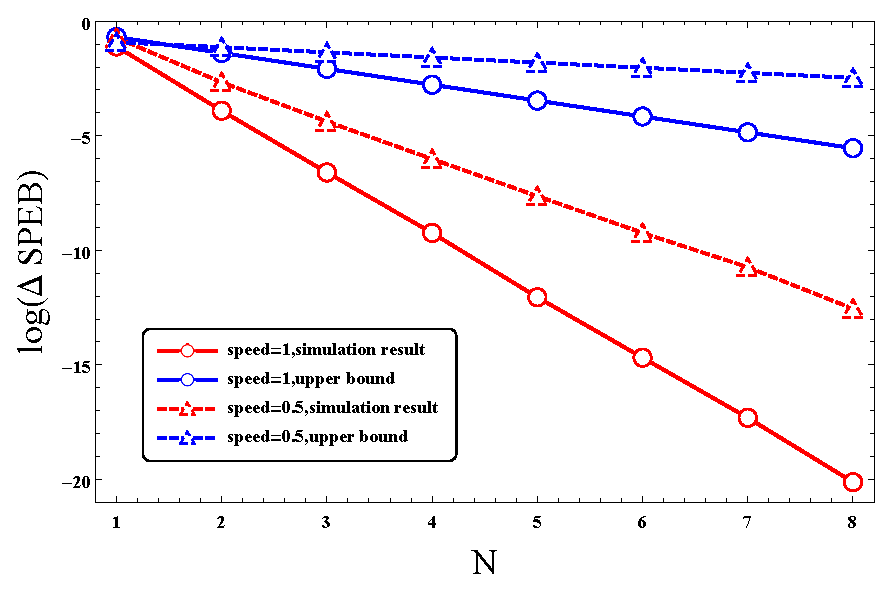
\includegraphics[width=0.4\textwidth]{decreasing_exponential.eps}
\caption{relationship between SPEB and time nodes used to locate the current node}\label{FF2}
\end{figure}

From this figure, we can see that the expectation of actual $\Delta$ SPEB decreases exponentially, much faster than the upper bound.
Another observation is that the faster the mean speed is, the less those distant time nodes contribute.
\section{Conclusion}
In this paper, we have discussed the temporal decaying characteristics of localization error. 
We use the method of continued fraction analysis to derive the exponential decaying property of the localization error. 
Our result gives insight on the relationship between localization error and cooperative information 
and can be applied to spatial  cooperation network without loop.


\begin{thebibliography}{1}
\bibitem{Win2011Network}
M.~Z. Win, A.~Conti, S.~Mazuelas, Y.~Shen, W.~M. Gifford, D.~Dardari, and
  M.~Chiani, ``Network localization and navigation via cooperation,''
  \emph{IEEE Communications Magazine}, vol.~49, no.~5, pp. 56--62, 2011.

\bibitem{6237577}
I.~Sharp, K.~Yu, and M.~Hedley, ``On the GDOP and accuracy for indoor
  positioning,'' \emph{IEEE Transactions on Aerospace and Electronic Systems},
  vol.~48, no.~3, pp. 2032--2051, JULY 2012.

\bibitem{LimitBound2}
Y.~Shen, H.~Wymeersch, and M.~Z. Win, ``Fundamental limits of wideband
  localization --- part ii: Cooperative networks,'' \emph{IEEE Transactions
  on Information Theory}, vol.~56, no.~10, pp. 4981--5000, Oct. 2010.
\bibitem{7887727}
Y.~Xiong, N.~Wu, and H.~Wang, ``On the performance limits of cooperative
  localization in wireless sensor networks with strong sensor position
  uncertainty,'' \emph{IEEE Communications Letters}, vol.~21, no.~7, pp.
  1613--1616, July 2017.
\bibitem{7962761}
Y.~Xiong, J.~Kuang, Y.~Feng, H.~Wang, and N.~Wu, ``Understanding the efficiency
  of cooperation in location-aware wireless networks,'' in \emph{2017 IEEE
  International Conference on Communications Workshops (ICC Workshops)}, May
  2017, pp. 828--833.


\bibitem{K2008Explicit}
E.K, ``Explicit formula for the inverse of a tridiagonal matrix by
  backward continued fractions,'' \emph{Applied Mathematics \& Computation},
  vol. 197, no.~1, pp. 345--357, 2008.

\end{thebibliography}

\end{document}
